\chapter{Related Work}\label{ch:related_work}

The wider community is well aware of the problem space created by untrusted/unreliable
code running inside the kernel and there have been a variety of attempts to deprivilege
components and/or improve the performance in networking-focused systems.
In \autoref{s:async} we explore new asynchronous APIs to minimise the system call overhead. In 
\autoref{s:userspace_dd} we examine user level I/O frameworks that bypass the OS altogether
to deprivilege device drivers and remove the system call overhead. Finally, in \autoref{s:isolation_dd}
we consider isolation techniques that take advantage of hardware virtualisation support to remove
drivers from the TCB.

\section{Asynchronous I/O Frameworks}\label{s:async}
In order to combat the performance overheads of typical network packet processing, a number of new APIs
have been developed with an asynchronous programming model.

\subsection{Netmap}\label{netmap}
Netmap aims to decrease packet processing costs on monolithic kernels through an asynchronous, zero copy 
API \cite{Rizzo_12}. Specifically, netmap removes the cost of dynamically allocating buffers per packet by 
preallocating fixed size packet buffers when the network device is first opened. These buffers are
shared between kernel and user space to remove the cost of data copying operations. Finally,
netmap removes the cost of blocking system call operations by providing an asynchronous API to user level applications. 
Applications open a special device file \lstinline{/dev/netmap} using \emph{ioctl()} and a flag to indicate registration.
This function will return the size of the memory region containing shared data structures for buffer management.  
On the receive path, another \emph{ioctl()} system call with the receive flag will return the number of packets available 
for reading. These packets can then be found in buffers ready to be dequeued from a shared receive queue. 
On the transmit path, applications write packets intended for transmit into shared buffers and insert into the shared transmit 
queue. Another \emph{ioctl()} system call is used with the transmit flag to notify the OS about the new 
packets to send. Importantly, the \emph{ioctl()} call with either the receive or transmit flag is non blocking.
This asynchronous interface is able to significantly reduce the system call overhead by providing a simple mechanism
to batch packet processing. With this, the netmap API achieves significantly higher transmit throughput than the
socket API.

\subsection{io\_uring}\label{io_uring}
\lstinline{io_uring} is another asynchronous API for I/O frameworks on Linux \cite{io_uring}. 
As opposed to netmap, \lstinline{io_uring} provides a more generalised interface for different 
classes of I/O processing and not just network-based applications. \autoref{f:fio_uring} shows the 2 shared
ring buffers between kernel and user space: one for submitting a request, another for results of completed requests. 
These ring buffers are set up using \emph{io\_uring\_setup()} and then mapped into user space with \emph{mmap()}. 
To issue a read or write request, applications must provide a user level buffer, set appropriate flags in the submission
queue entry and add this entry to the tail of the requests ring buffer. User applications inform
the kernel of updates to the requests ring buffer using a new system call \emph{io\_uring\_enter()}. This system call is blocking, 
and returns once the kernel has processed the new requests and the results are available in the completed queue. 
To provide an asynchronous interface, there is an optional polling mode, whereby the kernel will continue to poll for updates
in the requests queue. Polling mode removes the need for system calls, which can significantly improve throughput.

\begin{figure}[h]
	\centering
	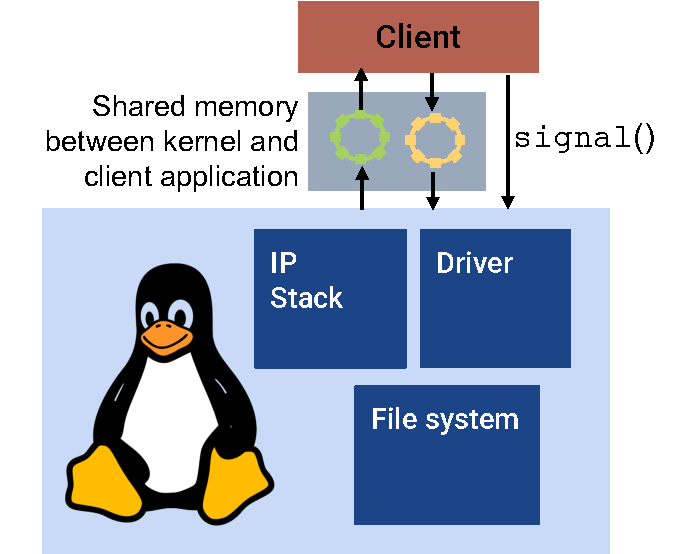
\includegraphics[width=7cm]{io_uring.pdf}
	\caption{System design with io\_uring.}
	\label{f:fio_uring}
  \end{figure}

\subsection{Takeaways}
Both netmap \cite{Rizzo_12} and \lstinline{io_uring} \cite{io_uring} reduce performance overheads of I/O on monolithic kernels
by providing an asynchronous interface to enable batching, or the complete removal of system calls. However, both APIs 
rely on in-kernel device drivers and do not explore the security vulnerabilities of such a design. 
Furthermore, netmap requires exclusive device access and thus the usual in-kernel device sharing mechanisms do not work. 
Instead, if the NIC is to be shared, the pool of data buffers will be mapped into every user process that shares the NIC. 
The result is that a process has access to data belonging to other processes. Also, the polling mode of
\lstinline{io_uring} would monopolise the CPU even when there is no work to be done, consequently driving up
power consumption of the system and it is unclear what policy is applied to this mode when there are multiple client
applications using it, or if there is other work to be done by the kernel.

\section{User space device drivers}\label{s:userspace_dd}
Running device drivers as user level programs is the simplest way to deprivilege the software and provide
strong fault isolation. However, this can lead to a significant increase in the number of system calls
required and this cost can degrade performance significantly. In order to overcome this, kernel bypass
frameworks have been developed to support user level IO asynchronously.

\subsection{DPDK}\label{dpdk}
DPDK (Data Plane Development Kit) provides data management libraries along with a set of network drivers to offload
network packet processing to user space and bypass the OS in a Linux environment \cite{DPDK:wp_20}. \autoref{f:dpdk}
shows the system design differences between using an in kernel network driver vs a DPDK library.

\begin{figure}[h]
  \centering
  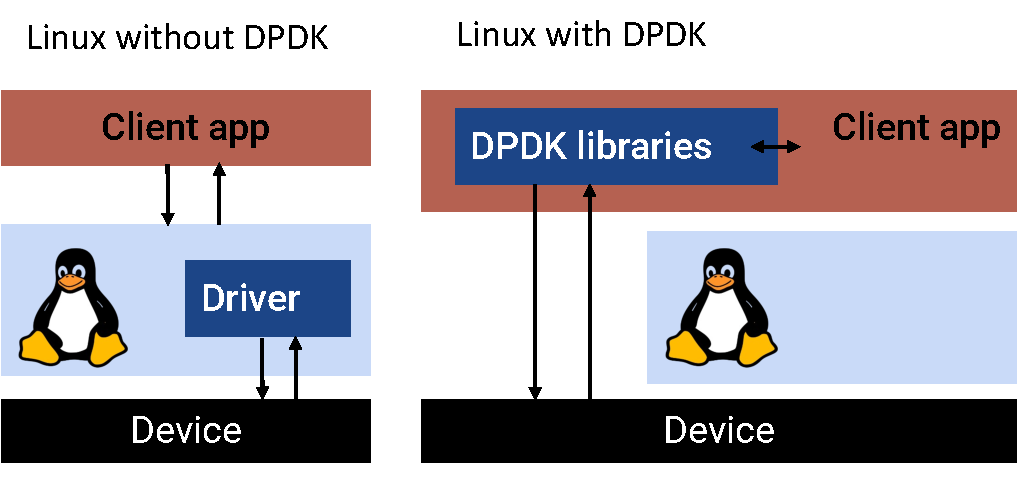
\includegraphics[width=10cm]{dpdk.pdf}
  \caption{System design without and with DPDK.}
  \label{f:dpdk}
\end{figure}

Specifically, it provides \cite{DPDK:wp_20}:
\begin{itemize}
	\item Lock free, bounded, multi producer, multi consumer (MPMC) ring buffer queues for efficient data management.
	\item Buffer management to preallocate fixed sized buffers.
	\item A library of polling mode drivers.
\end{itemize}

DPDK enables faster packet processing than a typical in-kernel driver as it removes the cost of context switching
between kernel and user space. Instead of receiving an interrupt, drivers must poll for hardware events. 
This means the driver needs to continuously read the device's event register. This has the consequence of driving
the CPU utilisation of the system up as the system cannot be idle while waiting for an event. 
In addition, the framework itself is zero copy, so DPDK can further reduce packet processing costs as it no longer needs to copy 
packet data into and out of user space. Finally, the framework uses huge pages for large memory pools, 
which decreases the amount of look-ups and other page management costs while ensuring relevant pages stay pinned in memory and
aren't migrated in the background due to Linux's page migration policy.

\subsubsection{BBQ}
BBQ is a block-based bounded queue design that aims to increase performance of ring buffer queues in frameworks such
as DPDK \cite{Wang_BFOOLCHC_22}. DPDK uses multi producer, multi consumer queues, which are designed with the
intention to split the workload across several processors. However, these queues have cache interference when
performing consecutive operations and this degrades performance. This stems from the MPMC queue design as it needs to keep track of
two heads and two tails to keep track of where a producer can produce to without interference from another producer (and
likewise for consumers). Pseudo code for interacting with MPMC queues is shown \autoref{l:prod} and \autoref{l:cons} 
\cite{Wang_BFOOLCHC_22}.

\noindent\begin{minipage}{.45\textwidth}
\fontsmall
\begin{lstlisting}[numbers=left, tabsize=2, language=C, caption={Producer pseudo code},frame=tb, label={l:prod}, captionpos=b]
  enqueue(data) {
  again:
  	ph = load(prod.head)
  	pn = ph + 1
  	if (pn > load(cons.tail) + SIZE)
  		return FULL
  	if (!cas(prod.head, ph, pn))
  		/* Another producer is 
  		   using this slot */
  		goto again
  	entry[pn] = data
  	/* Wait until earlier slots have
  	   successfully committed */
  	while(load(prod.tail) != ph)
  	store(prod.tail, pn)
  	return OK
  }
\end{lstlisting} 
\end{minipage}\hfill
\begin{minipage}{.45\textwidth}
\fontsmall
\begin{lstlisting}[numbers=left, tabsize=2, language=C, caption={Consumer pseudo code},frame=tb, label={l:cons}, captionpos=b]
  dequeue() {
  again:
  	ch = load(cons.head)
  	cn = ch + 1
  	if (cn > load(prod.tail))
  		return EMPTY
  	if (!cas(cons.head, ch, cn))
  		/* Another consumer is 
  		   consuming this slot */
  		goto again
  	data = entry[cn]
  	/* Wait until earlier slots have 
       successfully committed */
  	while(load(cons.tail) != ch)
  	store(cons.tail, cn)
  	return data
  }
\end{lstlisting}
\end{minipage}

The performance degradation comes from two possible places:
\begin{enumerate}
\item Cache misses occur in a multiprocessing environment every time a producer reads the
consumer's tail (on line 5 in \autoref{l:prod}), even though the tail might be far behind and not
of concern. This is because the cache belonging to the core running the producer will not have the
required data and it must be fetched from the owner (either from main memory or the local cache of
a core running a consumer). Likewise, the consumer will also always miss on the 
producer's tail (on line 5 in \autoref{l:cons}) although it may be far ahead.
\item When multiple threads try to read the same entry, they must continuously try again as shown at lines 7 - 10 in 
\autoref{l:prod} and \autoref{l:cons}
\end{enumerate}

BBQ proposes a block-based approach instead, where the queues are divided into blocks and the producers only
start using a block once it has been fully consumed. This avoids the cache miss on 
reading the consumer's tail. Each block contains 4 variables to keep track of the actions: allocated,
committed, reserved and consumed. Producers produce between allocated and committed, but these variables 
aren’t updated until the block is fully consumed (this is to prevent cache misses by the consumer).
Compared with DPDK, BBQ isn't as affected by CPU over-subscription. This is because in the MPMC
DPDK queues, the producers can form a waiting chain, where the last thread to allocate an entry can only 
commit that entry once the previous thread has committed its entry. While this waiting chain would have 
minimal impact if the threads are scheduled in the optimal order to each make progress, this is often not 
the case. As producers in BBQ commit independently using an atomic Fetch-and-Add 
instruction, this scenario does not occur.\\
Overall, the BBQ approach attempts to solve performance issues of MPMC queues in a multiprocessing environment,
which stem from the concurrency involved in such queues. 

\subsubsection{CleanQ}
CleanQ takes the opposite approach of BBQ and instead outlines the need for a simple and \emph{reliable} ring buffer
design that does not impede performance in frameworks such as DPDK \cite{Haecki_HACSR_19}. CleanQ removes
the inherent complexity of MPMC queues and instead returns to single producer, single consumer (SPSC)
queues. These queues are significantly simpler, and as a result, Haecki et. al. are able to infer
correct guarantees from the design. CleanQ uses the concept of `ownership' to base their formal invariants. 
Consider `entities' to be either a producer or a consumer acting on the queues and `objects' to be items passed around
by these queues, then the invariants guaranteed by the CleanQ design are:
\begin{enumerate}
\item An object has at most one owner,
\item If an entity owns an object, it has exclusive use of it,
\item An entity knows whether it owns an object or not,
\item Ownership can be transferred.
\end{enumerate}
These guarantees eliminate many subtle bugs in lock-free queue design.
Furthermore, the CleanQ design achieves higher throughput than DPDK MPMC queues in a networking
context, which ultimately highlights that a simple design does not negatively impact performance.

\subsubsection{Takeaways}
DPDK completely bypasses the OS to offload packet processing to user space. The zero copy design in user space
achieves higher throughput than typical in-kernel packet processing\cite{DPDK:wp_20}. However, all drivers 
are polling mode only. This design decision stems from the high cost of interrupt handling on Linux, but it enables
the application to monopolise the CPU as the driver must continuously poll for events. While the polling has little
impact in high throughput networking scenarios where there is consistently work to be done, at lower throughput,
the CPU utilisation will not decrease with the workload and the system will maintain high power consumption without
making progress. Moreover, implementing a device driver as a library inside an application limits the device to a
single client. Ultimately, the short-comings of monolithic kernels, namely, the high cost of interrupt processing
and context switching, have influenced the design and reduced the flexibility. DPDK also relies on cache-coherent
architectures to achieve performance, as the minimal support available for cache management operations from userspace
introduces costly system calls. Finally, MPMC queues used in the DPDK data plane are inherently complex due to the 
concurrency involved and have the potential to degrade performance \cite{Wang_BFOOLCHC_22}. The simpler and
cleaner design of ring buffer queues as shown in CleanQ, can not only achieve higher throughput, but are also
verifiable \cite{Haecki_HACSR_19}.

\subsection{Ixy}
Ixy is a user-space packet framework on Linux that aims to educate developers on driver development 
\cite{Emmerich_PBHZC_19}. It utilises the \emph{uio} and \emph{vfio} interfaces to access the device from
user space. Using these APIs, Ixy develops a user space polling mode device driver for the ixgbe 10Gbps
NIC with low packet forwarding costs. Significantly, the ixy device driver reduces the \emph{ixgbe}
in-kernel driver from over 10K LOC to just over 1K LOC.

\subsubsection{Linux uio}
\emph{uio} (User space I/O) exposes interfaces for user level device drivers by memory mapping files in the \emph{sysfs}
pseudo file system on Linux \cite{UIO}. Interrupts are handled by reading this file once mapped. For example,
a \emph{read()} system call will block until an interrupt is triggered. The integer value read from this file represents
the total interrupt count. \emph{uio} exposes the device registers via \emph{mmap()} when using a particular offset calculated
based on the number of devices using \emph{uio}. However, \emph{uio} hides the issue that DMA 
addresses must stay in resident memory and that Linux page migration does not guarantee that physical addresses
won't change behind the scenes. To overcome this issue, \emph{uio} users can use
huge pages as these won't be migrated by the Kernel.

\subsubsection{Linux vfio}
\emph{vfio} (Virtual Function I/O) extends \emph{uio} and adds support for IOMMU use \cite{VFIO}. The IOMMU is a memory
management unit mapping device-visible virtual addresses to physical addresses, and lies on the system bus between I/O devices
and main memory. When used, the main advantage of the IOMMU is protecting memory from malicious/faulty devices attempting
errant memory accesses. \emph{vfio} introduces additional
files in the \emph{sysfs} file system to expose the IOMMU to user space and provides data structures and library functions
that can be used to map/unmap memory in the IOMMU for safe DMA through \emph{ioctl()} system calls on Linux.

\subsubsection{Takeaways}
Although the ixy user level device driver is not as performant as its counterpart on the DPDK framework, it reduces a
large and complex device driver to a much smaller driver without significant performance degradation. The lower
performance of ixy when compared to DPDK can in part be attributed to DPDK's use of SIMD instructions to handle
batches of packets at a time \cite{Emmerich_PBHZC_19}. SIMD units are hardware components that perform the same
operation on multiple data operands concurrently. In packet processing, this parallelism can boost performance
on checksum calculations. However, much like DPDK, ixy is reliant on cache coherent architectures and also does
not support device sharing.

\subsection{Snap}\label{snap}
Snap proposes a modular architecture, comparable to a microkernel design, by utilising asynchronous communication
mechanisms and minimal state sharing \cite{Marty_dKAABCDDEGKKKMMORRSTVWV_19}. The design intentionally leans away 
from typical socket programming for networking systems and instead opts for an event driven model. They present
a user space network driver that uses asynchronous communication and ring buffers in shared memory for data transfer.
Interrupts are delivered to an event file, which can be polled from user
level. Alongside this, Snap takes a unique approach to scheduling. Rather than
designing a generic scheduling policy that aims to be applicable across a large set of scenarios, they instead propose 3
different designs that could be swapped as required:
\begin{enumerate} 
\item Tasks are pinned to cores to take advantage of cache efficiency.
\item Tasks are spread dynamically. Threads are scheduled when interrupts are delivered to process the event on
the next available core.
\item Tasks are spread dynamically as above but onto as few cores as possible. This aims to take advantage
of cache efficiency when possible, but as work queues up, the allocation needs to be queried. 
\end{enumerate}

\subsubsection{Takeaways}
The Snap design deprivileges untrusted drivers by running them in user space and the design, although running on top
of a monolithic kernel, uses event driven programming. This design is shown to scale well to multiple clients and the
swappable scheduling policy removes complexity from the trusted computing base while demonstrating efficiency.

\subsection{Microdrivers}
Instead of running the entire driver at user level, Microdrivers split the device driver into two separate
components; one of which runs at kernel level and the other at user level in order to achieve the performance 
of in kernel drivers combined with the fault isolation of user level drivers 
\cite{Ganapathy_RBSJ_08}. \autoref{f:microdrivers} shows the architecture of microdrivers. 
The kernel mode component contains performance critical and frequently used 
functionality. For a network driver, this includes interrupt handling and sending and 
receiving packets. The rest of the code, predominantly initialisation and error handling, goes into user level 
where the performance degradation of context switching between kernel and user level does not have noticeable
impact. In order to speed up the user mode component, microdrivers duplicate functions
in both components and use shared memory for frequently accessed data structures.

\begin{figure}[h]
  \centering
  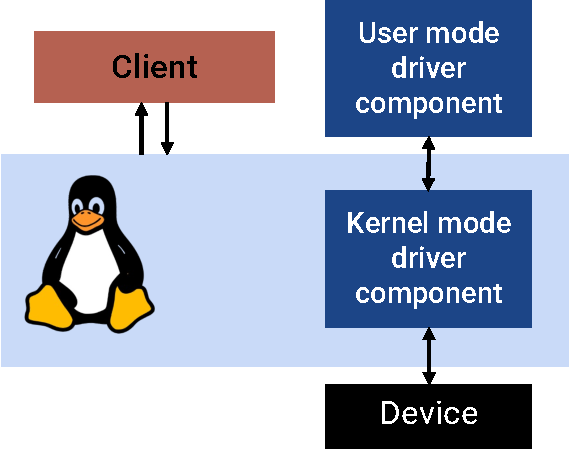
\includegraphics[width=8cm]{microdrivers.pdf}
  \caption{Microdrivers architecture}
  \label{f:microdrivers}
\end{figure}

\subsubsection{Takeaways}
Although 70\% of driver code consists of non-performance-critical functions and can be relegated to user space
\cite{Ganapathy_RBSJ_08}, this does not provide good fault isolation. The remaining 30\% of driver code is 
just as untrustworthy, and faults have higher impact as this code is on the critical path. Furthermore, by sharing
data structures between kernel and user space, some of which could contain sensitive kernel data, higher trust 
needs to be placed on the user mode component, thus diminishing any safety guarantees obtained by running the 
code at user level. Finally, the research was not able to produce reliable performance results which undermines
any performance gains of running part of the driver at kernel level. Thus, splitting a driver into a user level
component and a kernel level component is not viable and could achieve the worst of both designs: poor performance
and poor fault isolation.

%%%%%%%%%%%%%%%%%%%%%%%%%%%%%%%%%%%%%%%%%%%%%%%%%%%%%%%%%%%%%%%%%%%%%%%%%%%%%%%%%%%%%%%%%%%%%%%%%%%%%%%%%%%%%%%%%%%%%

\section{Isolating Kernel Components inside the OS}\label{s:isolation_dd}
Another method to deprivilege untrusted code inside the OS is to use isolation techniques. These approaches
rely on hardware virtualisation extensions in order to re-use legacy code and avoid the redesign and redevelopment
of OS components like drivers while also supporting device sharing.

\subsection{Nooks}
A Nook provides an isolated environment for driver execution inside a monolithic OS \cite{Swift_MLE_02}. The
driver still runs inside the kernel address space, but within a different protection domain. This can be achieved
using virtual memory protection and lowering the privilege level to remove access to privileged instructions. 
For shared resources, the OS can call into isolated device drivers with a wrapper function in order to track 
resource usage, verify data passed in/out, flush the TLB and perform a software trap. Similarly, a driver
accessing a shared data structure is trapped so the OS can update the data on the drivers behalf.

\subsubsection{Takeaways}
Unfortunately there is a lack of detail into the Nooks architecture and the work doesn't account for potential 
performance degradation due to some of the design decisions. Firstly, in order for the OS to update data on the drivers
behalf, it would need to first verify this data. How this data is verified and to what extent could cost cycles on a 
critical path. Furthermore, interrupts are forwarded to the isolated driver. Nooks measured 
interrupt handling on a isolated driver to cost double the cycles of an in kernel driver, yet 
there is no accounting for this in the performance. This cost is significant and would limit drivers to polling
mode only.

\subsection{{LXDs}}
LXDs (Lightweight Execution Domains) enable isolation in a monolithic OS using hardware-assisted virtualisation
(VT-x) \cite{Narayanan_BJSBQ_19}. The design utilises a small microkernel that runs inside the monolithic OS to
provide both synchronous and asynchronous communication channels between kernel processes and isolated components.
\autoref{f:lxds} outlines the architecture of this solution. Instead of a typical function call to transmit data 
that would call into an in-kernel driver library, it instead sends a message via the LXDs microkernel to the
isolated driver. The isolated driver has direct access to the NIC and can then perform the transmit. 

\begin{figure}[h]
  \centering
  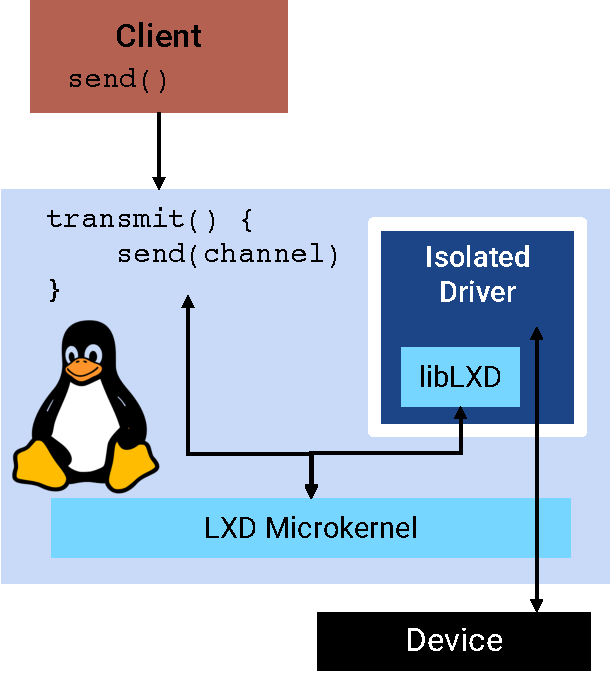
\includegraphics[width=7cm]{LXDs.pdf}
  \caption{System design of LXDs with an isolated NIC driver}
  \label{f:lxds}
\end{figure}

In order to achieve this design, they prescribe methods to decompose kernel code to help analyse the 
interaction patterns between the kernel and its drivers. They propose a new IDL (Interface Definition 
Language) to auto generate glue code based on these patterns. This glue code creates copies
of shared data structures to ensure such structures aren't shared between domains, and translates function calls into 
an isolated domain into remote procedure calls \cite{Narayanan_BJSBQ_19}.\\ 
To better isolate device drivers, the design pins a driver to a particular core and enables communication via cross-core
message passing. Synchronous message passing via the LXDs microkernel is used initially for establishing regions of
shared memory that are then set up for asynchronous communication in the form of ring buffer queues. Cross-core communication
then just relies on cache coherence, which has a lower cost (around 380 cycles) than using hardware mechanisms for
address space isolation (around 850 cycles)\\
Instead of blocking waiting for another core running an isolated driver to complete its work, the design proposes to instead
spawn a light weight thread when communicating asynchronously that can wait for the response. The original thread
can then keep executing. When this is not possible, for example, when the next instruction relies on the result of the call,
continuations can be used as well. 

\subsubsection{Takeaways}
Although the design was able to achieve throughput within 80\% of a non-isolated NIC driver,
the design has several limitations. Firstly, the design relies on utilising multiple cores to achieve comparable
performance. This is not always practical, and has the potential to waste resources. Although the paper does not display
CPU utilisation figures for their benchmarks, by pinning a polling driver to a particular core, even at low loads 
this core will be executing at 100\%. Additionally, the architecture involves adding a microkernel type
component to the trusted computing base inside the OS. Although it may be small, there is no comment on the
complexity of this new addition and this extra layer must be trusted in order to remove the driver from the TCB.
This design also introduces more concurrency into the kernel by spawning threads to wait for cross-core communication.
Finally, the research is limited to device drivers on multicore hardware and does not include other
layers and components in the networking processing plane such as the IP stack. The Linux kernel IP stack is significantly
more complex and difficult to isolate in such a manner.

\subsection{Isolation using VMFUNC}
Another method of isolating drivers and other kernel extensions is to use recent hardware mechanisms such as VMFUNC and
extended page table switching. This design involves executing the OS on top of a minimal hypervisor to make use of 
these hardware mechanisms \cite{Narayanan_HTJB_20}. VMFUNC is an Intel primitive that changes the extended page table
underneath a virtual machine without exiting into the hypervisor. As the VMFUNC instruction is significantly faster than
switching privilege levels, this research proposes using this instruction in a trampoline mechanism to quickly context switch
into an isolated component. \autoref{f:vmfunc} demonstrates the overall architecture. Similarly to the LXDs architecture,
the in kernel driver is replaced by stub code that crosses the isolation boundary using vmfunc trampoline code before
performing the transmit on the device.

\begin{figure}[h]
  \centering
  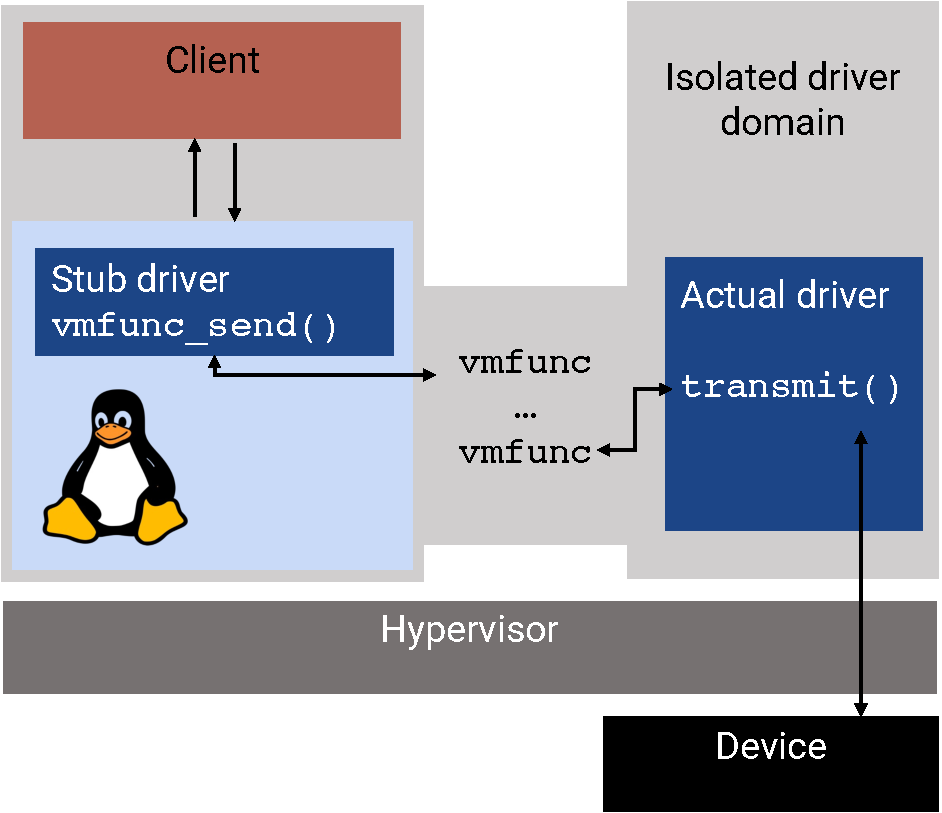
\includegraphics[width=10cm]{vmfunc.pdf}
  \caption{System design using vmfunc trampoline to isolate NIC driver}
  \label{f:vmfunc}
\end{figure} 

However, this architecture is not necessarily secure and extra measures must be taken. These are:
\begin{enumerate}
	\item Ensure virtual address spaces of isolated domains, kernel and user processes do not overlap. This is to prevent a 
	malicious component from executing VMFUNC on its own accord and having the ability to access to data it should not. 
	The same applies to physical addresses.
	\item ensure isolated domains have read-only access to their page table. This is to ensure an isolated component cannot
	change its address space layout and thus violate the above.
	\item Sensitive data is protected by either mediating it through the hypervisor (such as control registers) or saved and 
	restored across domain switches (general, segment and extended state registers). This happens in the trampoline code.
\end{enumerate}

\subsubsection{Takeaways}
Isolating a network driver using the above design achieved throughput within 1\% to 11\% of the native polling driver on a
10Gbps NIC. Although the isolation technique used seems to add minimal overhead, some overhead is hidden in the interrupt
delivery for non-polling drivers. The design proposes mapping the interrupt descriptor table is into both the kernel
and the isolated domains to prevent the need to trap into the hypervisor on interrupt. The interrupt is
then first handled by the kernel domain before interrupting the isolated driver where applicable. 
However, this allows an untrusted component access to the interrupt descriptor table and the ability to disable interrupts 
and never return control to the OS. To overcome this, they propose using a preemption timer in the hypervisor to ensure the 
kernel domain is making progress. Overall, the cost of delivering an interrupt to an isolated 
domain is over 1000 cycles, and the cost and trade-offs of using a preemption timer
in the hypervisor is not measured. Furthermore, to ensure an untrusted isolated component did not alter the interrupt
descriptor table without disabling all interrupts (eg. it could disable interrupts of some other device), the OS would
need to check the interrupt descriptor table on every return. This cost is not measured. Overall, mapping the interrupt
descriptor table into untrusted domains is inherently insecure and should be avoided. 

% RedLeaf? 
\section{Summary}
Typical network packet processing is both insecure and non-performant. This is because complex, bug prone software systems
run in the trusted computing base, and the complexity of such systems has led to reduced performance. The solutions outlined above
aim to rectify this, but are largely limited by the monolithic kernel design itself. 
Asynchronous IO frameworks improve performance without addressing the security vulnerabilities. User level drivers
achieve high throughput at the cost of high utilisation and are limited to single client applications. Although techniques to
isolate drivers inside the OS promote device sharing, these techniques are not extensible to other kernel subsystems, they
do not completely protect the OS and can also degrade performance. However, there are still some significant
learnings we can take away from the above work. Firstly, Rizzo (2012), Axboe (2019), Linux Foundation (2020) and Marty et al. (2019)
demonstrate significant performance gains through the use of an asynchronous API. Emmerich et al. (2019) showed that a complex
device driver for a high throughput NIC could be simplified 10 fold and still achieve performance. Haecki et al. (2019)
demonstrated that simple SPSC queues can outperform complex MPMC queues, and Marty et al. (2019) demonstrated that a
modularised approach with flexible policy achieves competitive throughput in a real world application of data centres.
